\documentclass[tikz,border=10pt]{standalone}
\usepackage{tikz}
\usetikzlibrary{arrows.meta, positioning, calc, shapes.geometric}
\usepackage{amsmath}
\usepackage{amssymb}

\begin{document}
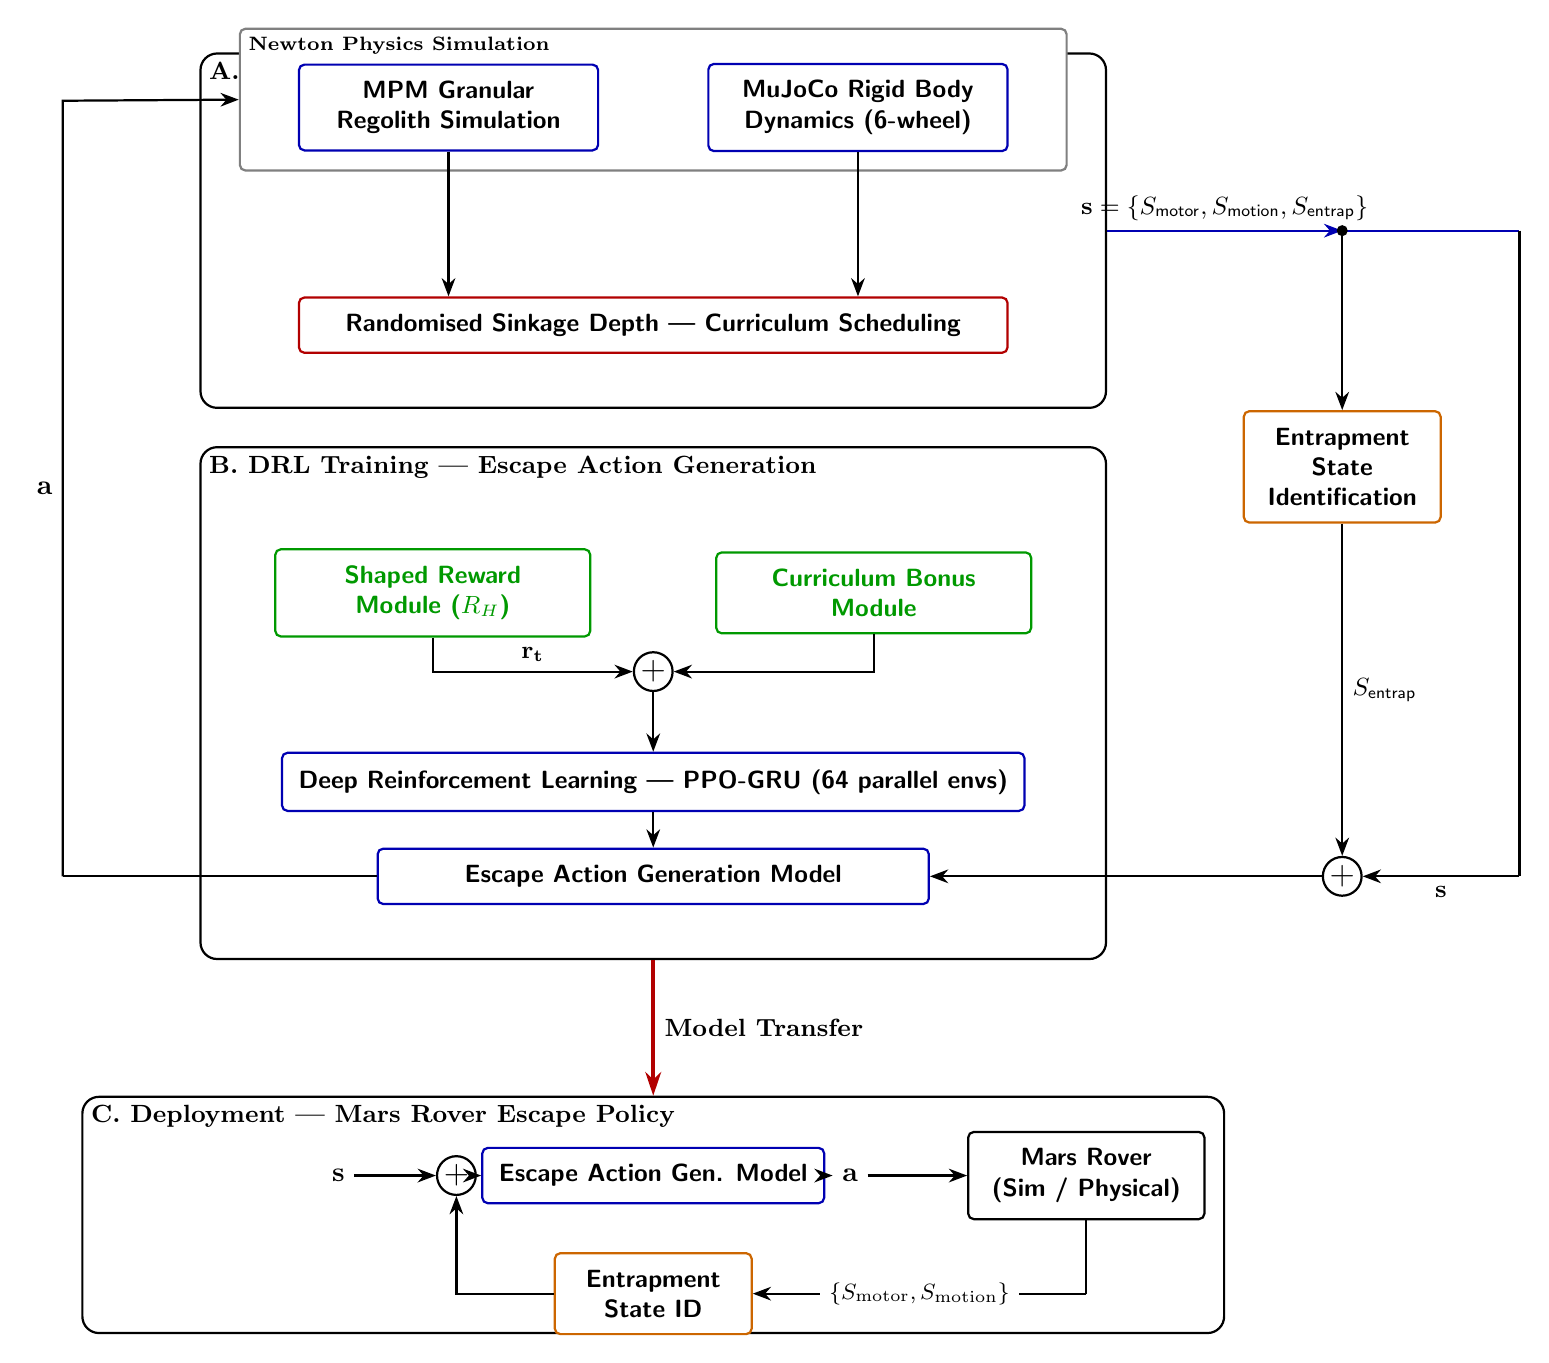
\begin{tikzpicture}[
    >=Stealth,
    font=\sffamily\small,
    box/.style={draw, thick, rounded corners=2pt, align=center, fill=white, inner sep=6pt},
    outerbox/.style={draw, thick, rounded corners=6pt, inner sep=10pt, fill=white},
    greenbox/.style={box, draw=green!60!black, text=green!60!black},
    bluebox/.style={box, draw=blue!70!black, text=black},
    redbox/.style={box, draw=red!70!black, text=black},
    orangebox/.style={box, draw=orange!80!black, text=black},
    plus/.style={circle, draw, thick, inner sep=0pt, minimum size=14pt, align=center, font=\large},
    arr/.style={->, thick}
]

% ================= BOX A: SIMULATION ENVIRONMENT =================
\node[outerbox, minimum width=11.5cm, minimum height=4.5cm] (boxA) at (0,9) {};
\node[anchor=north west, font=\small\bfseries] at (boxA.north west) {A. Mars Rover Operational Environment Simulation};

% Physics Sub-box
\node[box, draw=gray, minimum width=10.5cm, minimum height=1.8cm, yshift=-0.6cm] (physBox) at (boxA.north) {};
\node[anchor=north west, font=\scriptsize\bfseries] at (physBox.north west) {Newton Physics Simulation};

% Inner nodes of Physics Sub-box
\node[bluebox, minimum width=3.8cm] (mpm) at ($(physBox.center) + (-2.6, -0.1)$) {\textbf{MPM Granular} \\ \textbf{Regolith Simulation}};
\node[bluebox, minimum width=3.8cm] (mujoco) at ($(physBox.center) + (2.6, -0.1)$) {\textbf{MuJoCo Rigid Body} \\ \textbf{Dynamics (6-wheel)}};

% Curriculum Scheduling node
\node[redbox, minimum width=9cm] (sinkage) at ($(boxA.center) + (0, -1.2)$) {\textbf{Randomised Sinkage Depth --- Curriculum Scheduling}};

% Arrows inside Box A
\draw[arr] (mpm.south) -- (mpm.south |- sinkage.north);
\draw[arr] (mujoco.south) -- (mujoco.south |- sinkage.north);


% ================= BOX B: DRL TRAINING =================
\node[outerbox, minimum width=11.5cm, minimum height=6.5cm] (boxB) at (0,3) {};
\node[anchor=north west, font=\small\bfseries] at (boxB.north west) {B. DRL Training --- Escape Action Generation};

\node[greenbox, minimum width=4cm] (reward) at (-2.8, 4.4) {\textbf{Shaped Reward} \\ \textbf{Module ($R_H$)}};
\node[greenbox, minimum width=4cm] (bonus) at (2.8, 4.4) {\textbf{Curriculum Bonus} \\ \textbf{Module}};

\node[plus] (plusB) at (0, 3.4) {$+$};

\node[bluebox, minimum width=9cm] (drl) at (0, 2.0) {\textbf{Deep Reinforcement Learning --- PPO-GRU (64 parallel envs)}};

\node[bluebox, minimum width=7cm] (escapeB) at (0, 0.8) {\textbf{Escape Action Generation Model}};

% Arrows inside Box B
\draw[arr] (reward.south) |- (plusB.west) node[pos=0.75, above] {$\mathbf{r_t}$};
\draw[arr] (bonus.south) |- (plusB.east);
\draw[arr] (plusB.south) -- (drl.north);
\draw[arr] (drl.south) -- (escapeB.north);


% ================= BOX C: DEPLOYMENT =================
\node[outerbox, minimum width=14.5cm, minimum height=3cm] (boxC) at (0,-3.5) {};
\node[anchor=north west, font=\small\bfseries] at (boxC.north west) {C. Deployment --- Mars Rover Escape Policy};

\node[font=\bfseries] (sC) at (-4, -3) {$\mathbf{s}$};
\node[plus] (plusC) at (-2.5, -3) {$+$};
\node[bluebox, minimum width=4cm] (escapeC) at (0, -3) {\textbf{Escape Action Gen. Model}};
\node[font=\bfseries] (aC) at (2.5, -3) {$\mathbf{a}$};
\node[box, draw=black, minimum width=3cm] (roverC) at (5.5, -3) {\textbf{Mars Rover} \\ \textbf{(Sim / Physical)}};

\node[orangebox, minimum width=2.5cm] (entrapC) at (0, -4.5) {\textbf{Entrapment} \\ \textbf{State ID}};

% Arrows inside Box C
\draw[arr] (sC) -- (plusC);
\draw[arr] (plusC) -- (escapeC);
\draw[arr] (escapeC) -- (aC);
\draw[arr] (aC) -- (roverC);

% Feedback loop in Box C
\draw[thick] (roverC.south) -- (5.5, -4.5);
\draw[arr] (5.5, -4.5) -- (entrapC.east) node[midway, fill=white, font=\footnotesize] {$\{S_{\text{motor}}, S_{\text{motion}}\}$};
\draw[arr] (entrapC.west) -| (plusC.south);


% ================= GLOBAL CONNECTIONS & RIGHT SIDE =================

% Horizontal arrow from Box A — split at midpoint, extends to tip
\coordinate (split) at (8.75, 9);
\coordinate (hTip)  at (11.0, 9);

% Blue horizontal arrow: boxA.east → split → tip (label on first half)
\draw[->, thick, draw=blue!70!black]
    (boxA.east) -- (split)
    node[midway, above, text=black] {$\mathbf{s} = \{S_{\text{motor}}, S_{\text{motion}}, S_{\text{entrap}}\}$};
\draw[thick, draw=blue!70!black] (split) -- (hTip);

% Dot at midpoint (split)
\fill (split) circle (2pt);

% Entrapment Identification — below the midpoint
\node[orangebox, minimum width=2.5cm] (entrapA) at (8.75, 6) {\textbf{Entrapment} \\ \textbf{State} \\ \textbf{Identification}};

% Vertical arrow from midpoint → Entrapment block
\draw[arr] (split) -- (entrapA.north);

% Plus node for state concatenation
\node[plus] (plusRight) at (8.75, 0.8) {$+$};

% S_entrap: Entrapment block → top of +
\draw[arr] (entrapA.south) -- (plusRight.north) node[midway, right] {$S_{\text{entrap}}$};

% Bypass: from tip → down → left → right side of +
\draw[thick] (hTip) -- (11.0, 0.8);
\draw[arr]   (11.0, 0.8) -- (plusRight.east) node[midway, below] {$\mathbf{s}$};

% Input to Box B (State entry): + → escapeB right side
\draw[arr] (plusRight.west) -- (escapeB.east);

% Action feedback loop from Box B to Box A (Left side)
\draw[thick] (escapeB.west) -- (-7.5, 0.8);
\draw[arr] (-7.5, 0.8) -- (-7.5, 10.65) node[midway, left, font=\bfseries] {$\mathbf{a}$} -- (physBox.west);

% Model Transfer arrow
\draw[-{Stealth[length=3mm,width=2mm]}, draw=red!70!black, line width=1.5pt] (boxB.south) -- (boxC.north) node[midway, right, text=black, font=\bfseries\small] {Model Transfer};

\end{tikzpicture}
\end{document}
